\documentclass{article}
\usepackage{cmap}
\usepackage[utf8]{inputenc}
\usepackage[english,ukrainian]{babel}
\usepackage{graphicx}
\usepackage{geometry}
\usepackage{listings}
\usepackage{indentfirst}
\usepackage{subfigure}
\usepackage{caption}
\usepackage{amsmath}
\usepackage{float}
\geometry{
	a4paper,
	left=20mm,
	right=20mm,
	top=20mm,
	bottom=20mm
}
\lstset{
	extendedchars=\true,
	tabsize=4,
	language=python,
	showstringspaces=false,
	showtabs=false,
	frame=lrtb,
	columns=fixed,
	keepspaces,
	breaklines=true
}
\graphicspath{ {pictures} }
\setlength{\parindent}{4em}
\newcommand\subject{Чисельні методи}
\newcommand\lecturer{доцент кафедри ПЗ\\Мельник Н.Б.}
\newcommand\teacher{асистент кафедри ПЗ\\Гарматій Г.Ю.}
\newcommand\mygroup{ПЗ-16}
\newcommand\lab{7}
\newcommand\theme{Чисельні методи розв’язування систем нелінійних рівнянь}
\newcommand\purpose{Ознайомлення на практиці з методом ітерацій та методом Ньютона розв’язування систем нелінійних рівнянь}

\begin{document}
	\begin{large}
		\begin{titlepage}
			\thispagestyle{empty}
			\begin{center}
				\textbf{МІНІСТЕРСТВО ОСВІТИ І НАУКИ УКРАЇНИ\\
					НАЦІОНАЛЬНИЙ УНІВЕРСИТЕТ "ЛЬВІВСЬКА ПОЛІТЕХНІКА"}
			\end{center}
			\begin{flushright}
				Інститут \textbf{КНІТ}\\
				Кафедра \textbf{ПЗ}
			\end{flushright}
			\vspace{200pt}
			\begin{center}
				\textbf{ЗВІТ}\\
				\vspace{10pt}
				До лабораторної роботи № \lab\\
				\textbf{На тему}: “\textit{\theme}”\\
				\textbf{З дисципліни}: “\subject”
			\end{center}
			\vspace{90pt}
			\begin{flushright}
				
				\textbf{Лектор}:\\
				\lecturer\\
				\vspace{28pt}
				\textbf{Виконав}:\\
				
				студент групи \mygroup\\
				Коваленко Д.М.\\
				\vspace{28pt}
				\textbf{Прийняв}:\\
				
				\teacher\\
				
				\vspace{28pt}
				«\rule{1cm}{0.15mm}» \rule{1.5cm}{0.15mm} 2022 р.\\
				$\sum$ = \rule{1cm}{0.15mm}……………\\
				
			\end{flushright}
			\vspace{\fill}
			\begin{center}
				\textbf{Львів — 2022}
			\end{center}
		\end{titlepage}
		
		\begin{description}
			\item[Тема.] \theme.
			\item[Мета.] \purpose.
		\end{description}
		
		\section*{Теоретичні відомості}
		\subsection*{Метод простих ітерацій}
		Розглянемо систему двох нелінійних рівнянь з двома невідомими
		\begin{gather}
			\left\{\begin{array}{@{}l@{}}
				f_1(x, y)=0,\\\nonumber
				f_2(x,y)=0.\nonumber
			\end{array}\right.\,
		\end{gather}
		Розв’язком цієї системи є пара чисел $(x_*,y_*)$, яка перетворює систему рівнянь в тотожність.
		
		Припустимо, що $(x_0, y_0)$ - наближений розв’язок системи, яку
		перетворимо до такого вигляду
		\begin{gather}
			\left\{\begin{array}{@{}l@{}}
				x=\varphi_1(x, y),\\\nonumber
				y=\varphi_2(x,y).\nonumber
			\end{array}\right.\,
		\end{gather}
		де $\varphi_1$, $\varphi_2$ неперервно-диференційовані функції за змінними $x$ та $y$.
		
		Розглянемо ітераційний процес
		\begin{gather}\nonumber
			\left\{\begin{array}{@{}l@{}}
				x_{n+1}=\varphi_1(x_n, y_n),\\\nonumber
				y_{n+1}=\varphi_2(x_n,y_n).\nonumber
			\end{array}\right.\,
			\hspace{28pt}
			n=1,2,3...
		\end{gather}
		який породжує числові послідовності $\{x_n\}, \{y_n\}$
		
		Якщо ітераційний процес збігається, тобто існують границі
		\begin{gather}
			x_* = \lim_{n\rightarrow\infty}x_n,
			\hspace{28pt}
			y_* = \lim_{n\rightarrow\infty}y_n\nonumber
		\end{gather}
		то, систему рівнянь перепишемо у такому	вигляді
		\begin{gather}
			\left\{\begin{array}{@{}l@{}}
				x_*=\varphi_1(x_*, y_*),\\\nonumber
				y_*=\varphi_2(x_*,y_*).\nonumber
			\end{array}\right.\,
		\end{gather}
		тобто $x_*$, $y_*$ є розв’язком системи.
		\subsection*{Метод Ньютона}
		Розглянемо систему рівнянь
		\begin{gather}
			\left\{\begin{array}{@{}l@{}}
				f_1(x + \varDelta_x, y + \varDelta_y) = 0,\\\nonumber
				f_2(x + \varDelta_x, y + \varDelta_y) = 0.\nonumber
			\end{array}\right.\,
		\end{gather}
		Розкладемо функції $f_1$ і $f_2$ в ряд Тейлора, обмежившись лінійними членами розкладу відносно $\varDelta_x$, $\varDelta_y$
		\begin{gather}
			\left\{\begin{array}{@{}l@{}}
				f_1(x_0, y_0) + \frac{\partial f_1}{\partial x}\varDelta_x + \frac{\partial f_1}{\partial y}\varDelta_y = 0,\\\nonumber
				f_2(x_0, y_0) + \frac{\partial f_2}{\partial x}\varDelta_x + \frac{\partial f_2}{\partial y}\varDelta_y = 0.\nonumber
			\end{array}\right.\,
		\end{gather}
		Запишемо якобіан або визначник матриці Якобі, складеної з частинних
		похідних функцій $f_1$ і $f_2$ в деякій точці
		\begin{gather}
			\varDelta(x_0, y_0)=
			\begin{vmatrix}
				\frac{\partial f_1(x_0, y_0)}{\partial x} & \frac{\partial f_1(x_0, y_0)}{\partial y}\\
				\frac{\partial f_2(x_0, y_0)}{\partial x} & \frac{\partial f_2(x_0, y_0)}{\partial y}
			\end{vmatrix}
			\nonumber
		\end{gather}
		а поправкиx $\varDelta_x$ і $\varDelta_y$ визначимо за правилом Крамера із системи.
		\begin{gather}
			\varDelta_x=-\frac{1}{\varDelta(x_0,y_0)}
			\begin{vmatrix}\nonumber
				f_1(x_0,y_0) & \frac{\partial f_1(x_0, y_0)}{\partial y}\\
				f_2(x_0, y_0) & \frac{\partial f_2(x_0, y_0)}{\partial y}
			\end{vmatrix}\\\nonumber
			\varDelta_y=-
			\frac{1}{\varDelta(x_0,y_0)}
			\begin{vmatrix}
				\frac{\partial f_1(x_0, y_0)}{\partial x} & f_1(x_0, y_0)\\
				\frac{\partial f_2(x_0, y_0)}{\partial x} & f_2(x_0, y_0)
			\end{vmatrix}\nonumber
		\end{gather}
		
		Наступне наближення розв'язку системи отримаємо у вигляді
		\begin{gather}
			\left\{\begin{array}{@{}l@{}}
				x_{n+1} = x_n + \varDelta_x,\\\nonumber
				y_{n+1} = y_n + \varDelta_y.\nonumber
			\end{array}\right.\,
			\hspace{28pt}
			n=1,2,3...
		\end{gather}
		\section*{Лабораторне завдання}
		Розв'язати систему нелінійних рівнянь з точністю $\varepsilon=10^{-3}$ методом ітерацій та методом Ньютона.
		\begin{gather}
			\left\{\begin{array}{@{}l@{}}
				sin(x+2)-y=1.5,\\\nonumber
				x+cos(y-2) = 0.5.\nonumber
			\end{array}\right.\,
		\end{gather}
		\section*{Хід роботи}
		\subsection*{Метод простих ітерацій}
		\begin{figure}[h!]
			\centering
			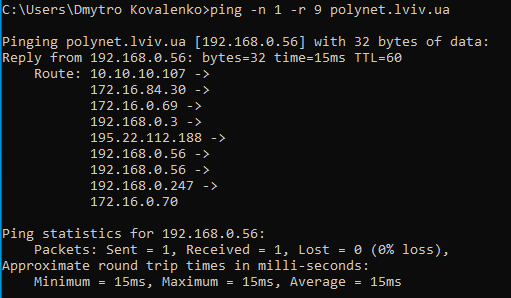
\includegraphics[scale=0.5]{3}
			\caption{Графік системи}
		\end{figure}
		Корінь рівняння лежить на проміжку $x\in[1, 2]$ та $y\in[-1, -2]$.
		За початкове наближення виберу $x_0 = 1$, $y_0 = -1$.
		
		Перетворю систему до такого вигляду
		\begin{gather}
			\left\{\begin{array}{@{}l@{}}
				y=\varphi_1(x,y) = sin(x+2)-1.5,\\\nonumber
				x=\varphi_2(x,y) = 0.5-cos(y-2).\nonumber
			\end{array}\right.\,
		\end{gather}
		Перевірю збіжність
		\begin{gather}\nonumber
			\frac{\partial \varphi_1(x_0, y_0)}{\partial x} = cos(x+2),\\\nonumber
			\frac{\partial \varphi_1(x_0, y_0)}{\partial y} = 0,\\\nonumber
			\frac{\partial \varphi_2(x_0, y_0)}{\partial x} = 0,\\\nonumber
			\frac{\partial \varphi_2(x_0, y_0)}{\partial y} = sin(y-2).\nonumber
		\end{gather}
		\begin{gather}\nonumber
			|\frac{\partial \varphi_1(x_0, y_0)}{\partial x}| +
			|\frac{\partial \varphi_1(x_0, y_0)}{\partial y}| = 0 + |cos(x+2)| < 1,\\\nonumber
			|\frac{\partial \varphi_2(x_0, y_0)}{\partial x}| +
			|\frac{\partial \varphi_2(x_0, y_0)}{\partial y}| = 0+|sin(y-2)| < 1.\nonumber
		\end{gather}
		Отже, процес збіжний.
			
		\noindent\textit{\textbf{Код програми} (файл lab\_\lab1.py):}
		\begin{lstlisting}
from math import sin, cos

def phi(x, y):
	phi1 = 0.5 - cos(y-2)
	phi2 = sin(x+2) - 1.5
	return (phi1, phi2)

eps = 0.001
i = 0

def iteration_method(x, y):
	"""Метод простих ітерацій"""
	(x_new, y_new) = phi(x, y)
	global i
	i += 1
	print(f"i:{i}  X:[{round(x_new, 3)}, {round(y_new, 3)}]")
	if abs(x_new - x) + abs(y_new - y) < eps: 
		return
	else:
		return iteration_method(x_new, y_new)

print(iteration_method.__doc__)
iteration_method(1, -1)\end{lstlisting}

		\begin{figure}[H]
			\centering
			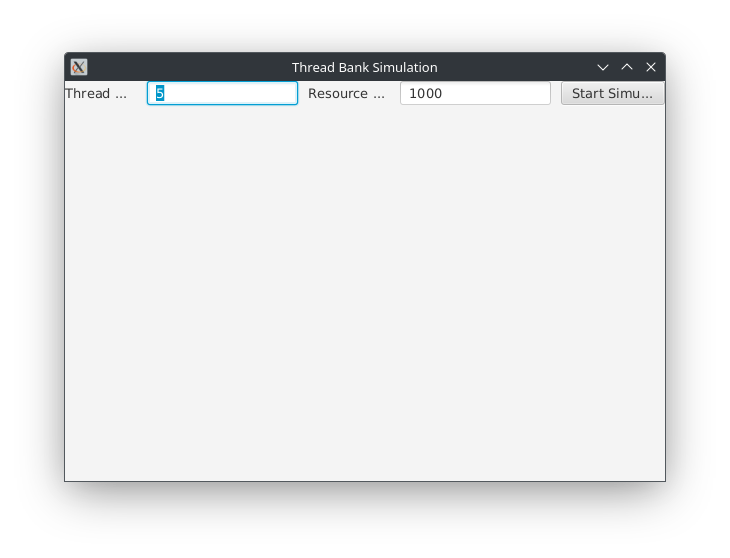
\includegraphics{1}
			\caption{Робота програми}
		\end{figure}
		
		\subsection*{Метод Ньютона}
		Якобіан системи
		\begin{gather}
			\varDelta(x_0, y_0)=
			\begin{vmatrix}
				\frac{\partial f_1(x_0, y_0)}{\partial x} & \frac{\partial f_1(x_0, y_0)}{\partial y}\\
				\frac{\partial f_2(x_0, y_0)}{\partial x} & \frac{\partial f_2(x_0, y_0)}{\partial y}
			\end{vmatrix}
			=
			\begin{vmatrix}
				-cos(x+2) & 1\\
				-1 & -sin(2-y)
			\end{vmatrix}
			\nonumber
		\end{gather}
		\noindent\textit{\textbf{Код програми} (файл lab\_\lab2.py):}
		\begin{lstlisting}
from numpy import array, linalg
from numpy.linalg import norm, inv as invert
from math import sin, cos

def newton_method(X, f, j, eps):
	"""Метод Ньютона"""
	print(newton_method.__doc__)
	for i in range(int(1e6)):
		deltaX = invert(j(X)) @ f(X)
		X -= deltaX 
		print(f"i:{i}  X:[{round(X[0], 3)}, {round(X[1], 3)}]")
		if norm(deltaX) < eps:
			break
	return X

def f(args):
	x, y = args
	return array((1.5 - sin(x+2) + y, 0.5 - cos(y-2) - x))

def j(args):
	x, y = args
	return array((
		(-cos(x+2), 1),
		(-1, -sin(2-y)),
	))

newton_method([1,-1], f, j, 10e-3)\end{lstlisting}
		
		\begin{figure}[H]
			\centering
			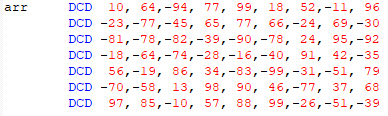
\includegraphics{2}
			\caption{Робота програми}
		\end{figure}
		
		\section*{Висновок}
		На лабораторній роботі я засвоїв практичні навички використання методу простих ітерацій та методу Ньютона та розробив функції для розв’язку системи нелінійних рівнянь з точністю $\varepsilon=10^{-3}$.
		Розв'язки системи рівнянь: $1.346; -1.703$.
		\begin{gather}
			\left\{\begin{array}{@{}l@{}}
				sin(x+2)-y=1.5,\\\nonumber
				x+cos(y-2) = 0.5.\nonumber
			\end{array}\right.\,
		\end{gather}

	\end{large}
\end{document}
